%! Author = zhiweizhang
%! Date = 11.06.25

% Preamble
\begin{figure}[ht]
    \centering
    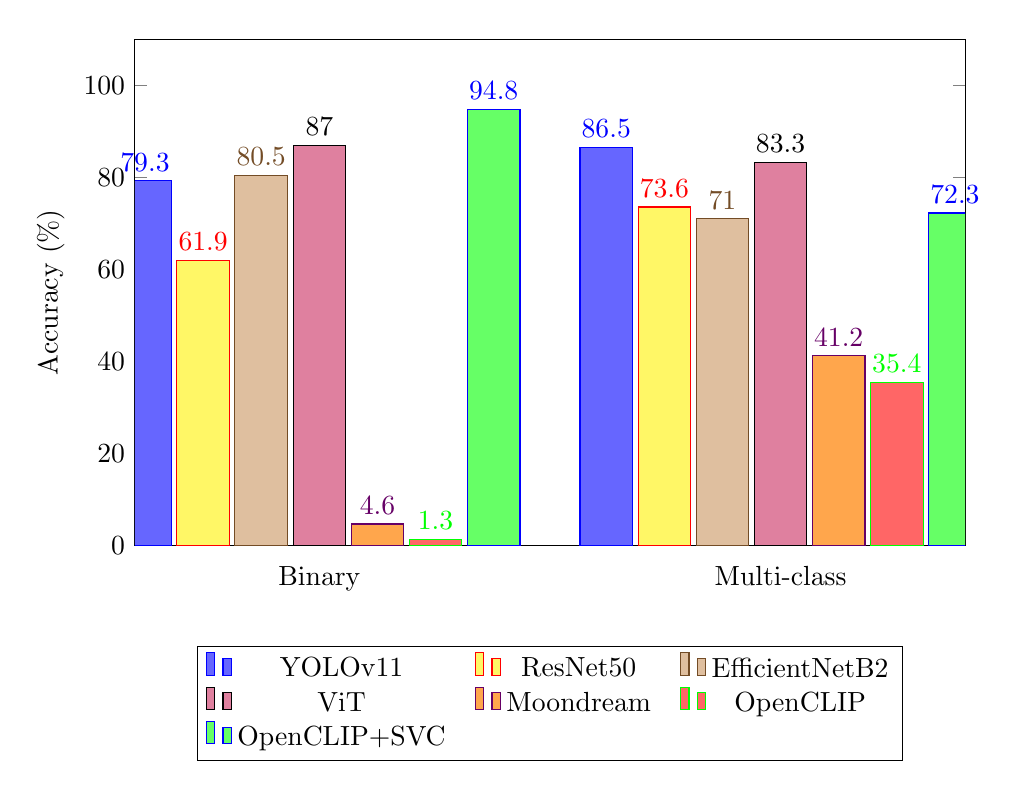
\begin{tikzpicture}
        \begin{axis}[
            ybar,
            bar width=19pt,
            width=\textwidth,
            height=8cm,
            enlarge x limits=0.4,
            ylabel={Accuracy (\%)},
            symbolic x coords={Binary, Multi-class},
            xtick=data,
            ymin=0.0, ymax=110.0,
            nodes near coords,
            nodes near coords align={vertical},
            major x tick style = transparent,
            legend style={
                at={(0.5,-0.2)},
                anchor=north,
                legend columns=3,
                /tikz/every even column/.append style={column sep=0.3cm}
            }
        ]
        \addplot+[style={fill=blue!60}]      coordinates {(Binary, 79.3) (Multi-class, 86.5)};
        \addplot+[style={fill=yellow!60}]    coordinates {(Binary, 61.9) (Multi-class, 73.6)};
        \addplot+[style={fill=brown!50}]     coordinates {(Binary, 80.5) (Multi-class, 71.0)};
        \addplot+[style={fill=purple!50}]    coordinates {(Binary, 87.0) (Multi-class, 83.3)};
        \addplot+[style={fill=orange!70}]    coordinates {(Binary, 4.6) (Multi-class, 41.2)};
        \addplot+[style={fill=red!60}]       coordinates {(Binary, 1.3) (Multi-class, 35.4)};
        \addplot+[style={fill=green!60}]     coordinates {(Binary, 94.8) (Multi-class, 72.3)};
        \legend{
            YOLOv11,
            ResNet50,
            EfficientNetB2,
            ViT,
            Moondream,
            OpenCLIP,
            OpenCLIP+SVC
        }
        \end{axis}
    \end{tikzpicture}
    \caption{Classification precision of selected models for binary and multi-class tasks.}
    \label{fig:model-precision}
\end{figure}